%%%%%%%%%%%%%%%%%%%%%%%%%%%%%%%%%%%%%%%%%%%%%%%%%%%%%%%%%%%%%%%%%%%%%%%%%%%%%%%
%                       CARREGA DE LA CLASSE DE DOCUMENT                      %
%                                                                             %
% Les opcions admissibles son:                                                %
%      12pt / 11pt            (cos dels tipus de lletra; no feu servir 10pt)  %
%                                                                             %
% catalan/spanish/english     (llengua principal del treball)                 %
%                                                                             % 
% french/italian/german...    (si necessiteu fer servir alguna altra llengua) %
%                                                                             %
% listoffigures               (El document inclou un Index de figures)        %
% listoftables                (El document inclou un Index de taules)         %
% listofquadres               (El document inclou un Index de quadres)        %
% listofalgorithms            (El document inclou un Index d'algorismes)      %
%                                                                             %
%%%%%%%%%%%%%%%%%%%%%%%%%%%%%%%%%%%%%%%%%%%%%%%%%%%%%%%%%%%%%%%%%%%%%%%%%%%%%%%

\documentclass[12pt,spanish,listoffigures,listoftables]{tfgetsinf}

%%%%%%%%%%%%%%%%%%%%%%%%%%%%%%%%%%%%%%%%%%%%%%%%%%%%%%%%%%%%%%%%%%%%%%%%%%%%%%%
%                     CODIFICACIO DEL FITXER FONT                             %
%                                                                             %
%    windows fa servir normalment 'ansinew'                                   %
%    amb linux es possible que siga 'latin1' o 'latin9'                       %
%    Pero el mes recomanable es fer servir utf8 (unicode 8)                   %
%                                          (si el vostre editor ho permet)    % 
%%%%%%%%%%%%%%%%%%%%%%%%%%%%%%%%%%%%%%%%%%%%%%%%%%%%%%%%%%%%%%%%%%%%%%%%%%%%%%%

\usepackage[utf8]{inputenc} 

%%%%%%%%%%%%%%%%%%%%%%%%%%%%%%%%%%%%%%%%%%%%%%%%%%%%%%%%%%%%%%%%%%%%%%%%%%%%%%%
%                        ALTRES PAQUETS I DEFINICIONS                         %
%                                                                             %
% Carregueu aci els paquets que necessiteu i declareu les comandes i entorns  %
%                                          (aquesta seccio pot ser buida)     %
%%%%%%%%%%%%%%%%%%%%%%%%%%%%%%%%%%%%%%%%%%%%%%%%%%%%%%%%%%%%%%%%%%%%%%%%%%%%%%%



%%%%%%%%%%%%%%%%%%%%%%%%%%%%%%%%%%%%%%%%%%%%%%%%%%%%%%%%%%%%%%%%%%%%%%%%%%%%%%%
%                        DADES DEL TREBALL                                    %
%                                                                             %
% titol, alumne, tutor i curs academic                                        %
%%%%%%%%%%%%%%%%%%%%%%%%%%%%%%%%%%%%%%%%%%%%%%%%%%%%%%%%%%%%%%%%%%%%%%%%%%%%%%%

\title{Interconexión del robot NAO a servicios de simulación en la nube}
\author{Carmona Vila, Jahel}
\tutor{Blanes Noguera, Juan Francisco}
\curs{2018-2019}

%%%%%%%%%%%%%%%%%%%%%%%%%%%%%%%%%%%%%%%%%%%%%%%%%%%%%%%%%%%%%%%%%%%%%%%%%%%%%%%
%                     PARAULES CLAU/PALABRAS CLAVE/KEY WORDS                  %
%                                                                             %
% Independentment de la llengua del treball, s'hi han d'incloure              %
% les paraules clau i el resum en els tres idiomes                            %
%%%%%%%%%%%%%%%%%%%%%%%%%%%%%%%%%%%%%%%%%%%%%%%%%%%%%%%%%%%%%%%%%%%%%%%%%%%%%%%

\keywords{NAO, simulador, diabetes, HTTP, MQTT} % Paraules clau 
         {NAO, simulador, diabetes, HTTP, MQTT} % Palabras clave
         {NAO, simulator, diabetes, HTTP, MQTT}        % Key words

%%%%%%%%%%%%%%%%%%%%%%%%%%%%%%%%%%%%%%%%%%%%%%%%%%%%%%%%%%%%%%%%%%%%%%%%%%%%%%%
%                              INICI DEL DOCUMENT                             %
%%%%%%%%%%%%%%%%%%%%%%%%%%%%%%%%%%%%%%%%%%%%%%%%%%%%%%%%%%%%%%%%%%%%%%%%%%%%%%%

\begin{document}

\begin{abstract}
En aquest projecte es desenvolupen serveis en el núvol per tal de desacoblar de dins del robot NAO el codi que executa el simulador de diabetes que duu implementat. Es suprimeixen les connexions TCP per protocols de capes superiors en la pila TCP/IP com son HTTP i MQTT que permeten una comunicació més flexible i amb més opcions. A més, es modernitza el codi de manera que sigue més senzilla tant la seva estructura com la seva compilació i execució.
\end{abstract}
\begin{abstract}[spanish]
En este proyecto se desarrollan servicios en la nube para desacoplar de dentro del robot NAO el código que ejecuta el simulador de diabetes que lleva implementado. Se suprimen las conexiones TCP por protocolos de capas superiores en la pila TCP/IP como son HTTP y MQTT que permiten una comunicación más flexible y con más opciones. Además, se moderniza el código para que sea más sencilla tanto su estructura como su compilación y ejecución.
\end{abstract}
\begin{abstract}[english]
In this project are developed cloud services to disengage the code inside the NAO Robot that starts up the diabetes simulator. TCP connectios are suppressed by higher layer protocols in the TCP/IP stack as HTTP and MQTT are which allow a more flexible communication and with more options. Besides the code is modernized so that this can be simplier in terms of structure, compilation and execution.
\end{abstract}

%%%%%%%%%%%%%%%%%%%%%%%%%%%%%%%%%%%%%%%%%%%%%%%%%%%%%%%%%%%%%%%%%%%%%%%%%%%%%%%
%                              CONTINGUT DEL TREBALL                          %
%%%%%%%%%%%%%%%%%%%%%%%%%%%%%%%%%%%%%%%%%%%%%%%%%%%%%%%%%%%%%%%%%%%%%%%%%%%%%%%

\mainmatter

%%%%%%%%%%%%%%%%%%%%%%%%%%%%%%%%%%%%%%%%%%%%%%%%%%%%%%%%%%%%%%%%%%%%%%%%%%%%%%%
%                                  INTRODUCCIO                                %
%%%%%%%%%%%%%%%%%%%%%%%%%%%%%%%%%%%%%%%%%%%%%%%%%%%%%%%%%%%%%%%%%%%%%%%%%%%%%%%

\chapter{Introducción}

\section{Motivación}

Este proyecto desarrollado parte directamente de <<\textit{Desarrollo de un sistema de monitorización y control de un robot simulador de diabetes}>>, un trabajo anterior a éste, el cual se encuentra en Riunet \cite{TFMAnterior}, elaborado por Antonio Bengochea Carrasco y dirigido también por Francisco José Blanes Noguera. Lo que se trata en el actual proyecto es de mejorar la infraestructura anterior teniendo en cuenta las limitaciones sobre las prestaciones que existen hoy en día para el proyecto previo. El centro del proyecto se encuentra dentro del robot NAO, por lo que es el que limita el crecimiento de la aplicación. \\

NAO es un robot humanoide programable y autónomo, desarrollado por Aldebaran Robotics, una empresa francesa con sede en París subsidiaria del grupo Softbank. Estos robots son ampliamente utilizados en por ejemplo la Robocup, un concurso de robótica a nivel internacional. \\

\begin{figure}[!h]
	\centering
	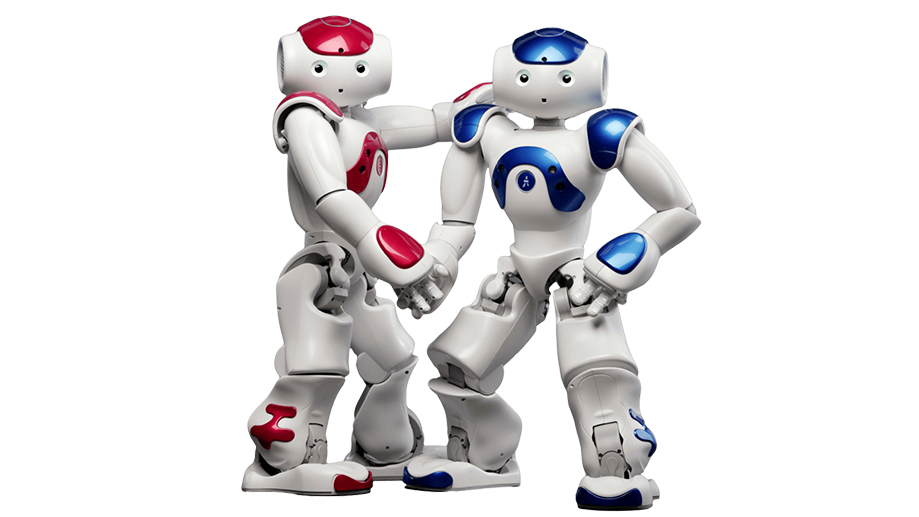
\includegraphics[height=5.5cm]{img/NAOIlustracion}
	\caption{Robot NAO en varios colores}
	\label{figura:NAOIlustracion}
\end{figure}

En esta hoja técnica \cite{NAOdatasheet} se detallan las características técnicas del robot que es objeto de estudio. Con unas dimensiones de 574x275x311mm y un peso de 5.4 kg, el robot consigue su movilidad mediante motores de corriente continua sin escobillas, siendo un total de 26 motores. En la imagen \ref{figura:NAOCinematica} podemos ver su esquema cinemático, en el cual se ven los ángulos de rotación y traslaciones. \\

\begin{figure}[!h]
	\centering
	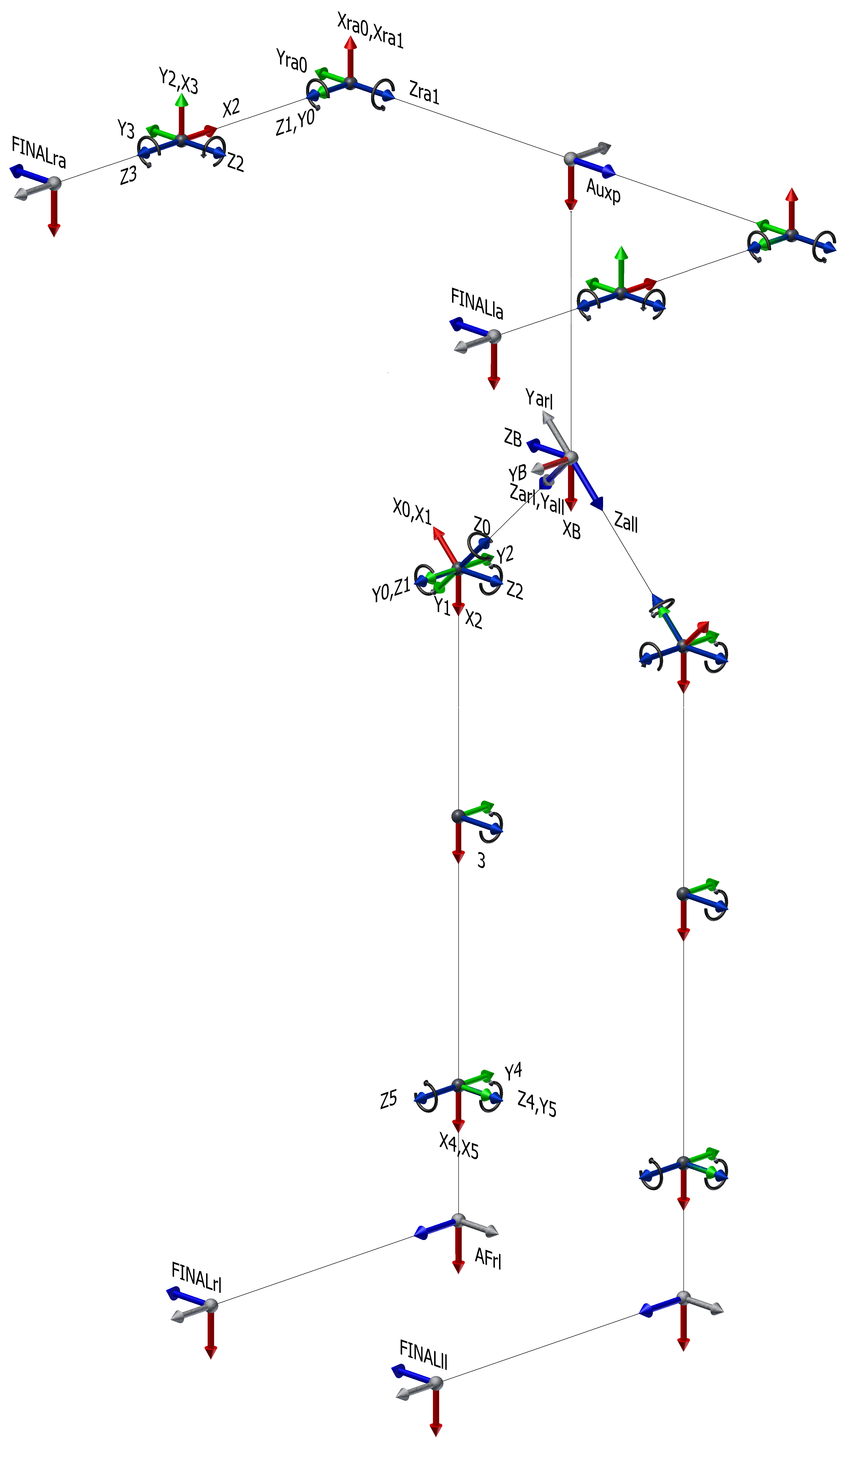
\includegraphics[height=10cm]{img/NAOCinematico}
	\caption{Esquema cinemático del robot NAO.}
	\label{figura:NAOCinematica}
\end{figure}

Como se ha mencionado antes, este proyecto parte de un proyecto anterior, cuyas limitaciones del propio robot suponen a su vez límites en el crecimiento de los procesos que lleva implementados. Precisamente, el componente que ejerce de tope es la unidad de cómputo y sus elementos asociados, como las memorias, o lo que el fabricante denomina \textit{Motherboard}. El límite es debido a que el robot incluye un simulador de diabetes que emplean librerías científicas. Esto supone un uso exhaustivo de los recursos de cómputo del robot, siendo que además del propio simulador, también corren otros procesos e hilos. Las características del robot para este aspecto podemos verlas en la tabla \ref{tabla:motherboardnao}: \\

\begin{table}[h]
\begin{center}
\begin{tabular}{|l|l|r|}
	\hline 
	\textbf{Elemento} & \textbf{Subelemento} & \textbf{Prestaciones} \\ 
	\hline 
	\textbf{CPU} & CPU Processor & Intel ATOM Z530 \\ 
	\hline 
	& Cache memory  & 512KB \\ 
	\hline 
	& Clock speed & 1.6GHz \\ 
	\hline 
	& FSB speed & 533MHz \\ 
	\hline 
	\textbf{RAM} &  & 1GB \\ 
	\hline 
	\textbf{Flash memory} &  & 2GB \\ 
	\hline 
	\textbf{Micro SDHC} &  & 8GB \\ 
	\hline 
\end{tabular} 
\caption{Motherboard del robot NAO}
\label{tabla:motherboardnao}
\end{center}
\end{table}

Para las aplicaciones de hoy en día, 1GB en memoria principal (RAM) es demasiado poco. Además teniendo en cuenta que aparte de ejecutar el código, que es muy cargante como hemos mencionado, también ejecuta otros procesos como por ejemplo la comunicación con sus actuadores y sensores mediante \textit{proxyes} como denomina el fabricante, o por ejemplo la comunicación via HTTP, SSH, entre otros. Por otra parte, el procesador Intel ATOM tienen un rendimiento bajo, como se muestra en a figura \ref{figura:IntelAtom}. No aparece el modelo de NAO, Atom Z530, pero el rendimiento es similar a los modelos que se muestran en la imagen. \\

\begin{figure}[!h]
	\centering
	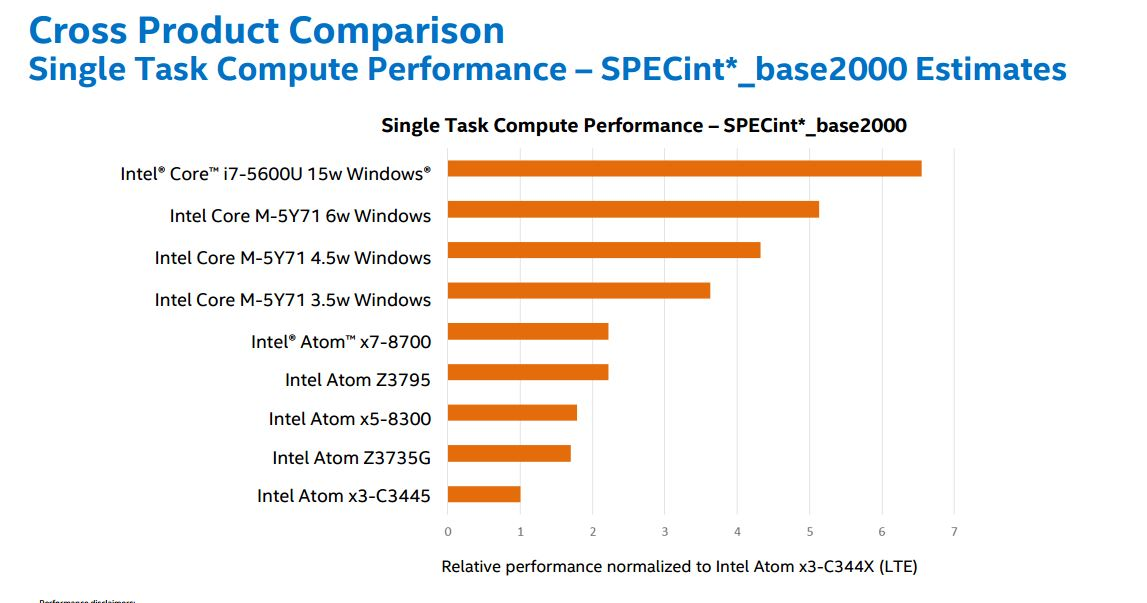
\includegraphics[height=7cm]{img/IntelAtom}
	\caption{Comparativa de rendimiento de procesadores Intel.}
	\label{figura:IntelAtom}
\end{figure}

Es importante entender que el modelo de comportamiento del páncreas que se sigue para simular la diabetes es el modelo \textbf{Hovorka}, cuya implementación puede encontrarse en sus documentos de investigación publicados, como por ejemplo \textbf{TODO: CITAR BIEN EL MODELO DE PANCREAS}. Su resolución pasa por ecuaciones diferenciales que se ejecutan periódicamente, lo cual resulta muy pesado para una máquina de las características que hemos observado.

\section{Repaso del proyecto anterior}

??????????????????

\section{Objetivo}

El objetivo de este proyecto es \textbf{desengarzar la parte pesada del código del anterior proyecto para virtualizarla en un servicio en la nube}. Esta parte es el simulador de diabetes, que implementa ecuaciones muy costosas computacionalmente y emplea librerías científicas. \\

Esto implica una transformación total de la parte del código de NAO, que significa actualizar las partes del proyecto <<\textit{Desarrollo de un sistema de monitorización y control de un robot simulador de diabetes}>>. Se ha eliminado complemtamente TCP de la estructura del proyecto y se ha sustituido por MQTT o HTTP (REST), según necesidad. Las partes del proyecto por lo tanto necesitan estas modificaciones: 
\begin{itemize}
	\item Aplicación Java: En vez de utilizar una conexión TCP para conectarse al robot, deberá utilizar librerías para hacer llamadas HTTP y un cliente MQTT. 
	\item La parte de NAO: Sufre un cambio radical ya que se debe cambiar de C++ a Python 2.7 \textbf{TODO: RELACIONAR CON LA PARTE QUE LO JUSTIFICO}(la versión que admite NAO), y se divide el proyecto en dos partes:
		\subitem -- Google Cloud Engine: Se debe alquilar un servicio en la nube, en este caso del proveedor Google, y se montará un servidor que atenderá peticiones HTTP. Las responderá con el status de la glucosa actualmente, ya que contendrá el simulador de diabetes.
		\subitem -- Código en NAO: Se debe eliminar toda la parte del simulador y TCP. Se añadirán dos librerías de HTTP y un cliente MQTT. 
\end{itemize}

\section{Estructura de la memoria}

Este proyecto se va a dividir en cuatro partes, que corresponden a las tres partes que conforman el proyecto y una cuarta sobre cómo se relacionan entre ellas. Las tres partes son las mencionadas en la sección anterior: Cliente Java, servicio en la nube y código en NAO. \\

Finalmente, se valorará el resultado del proyecto mediante unas conclusiones y se listarán una serie de posibles mejoras al proyecto actual. También hay un apéndice con información técnica acerca de cómo configurar los diferentes servicios.


\chapter{Servicio en la nube}

Idees de estructura:
- Explicació del NAO i tipos de llenguatge
- Explicació del projecte anterior i arquitectura (dibuixets de TCP)
- Explicació de les limitacions de còmput de NAO i de limitacions de TCP
- Estructura del meu projecte. MQTT entrar en detall del QoS. (Part Java, Part NAO i part GCloud).
- Part Java: Mínim canvi realment. Explicar Paho i que es un client Rest.
- Part NAO: Que he reconvertit el codi a Python perquè el NAO te molt mal el C++. 
- Part GCloud: Aquí explayar-se.
- Millores: Prescindir de GCloud i montarse una raspi amb un DNS, afegir més funcions al NAO, mes precisio del simulador aprofitant gcloud, manejar varios NAOs amb una sola app java i un sol gcloud...

\chapter{Código en NAO}

????? ????????????? ????????????? ????????????? ????????????? ?????????????

\chapter{Aplicación Java}

????? ????????????? ????????????? ????????????? ????????????? ?????????????

\chapter{Relación entre los componentes}

????? ????????????? ????????????? ????????????? ????????????? ????????????? 

\section{?? ???? ???? ? ?? ??}

????? ????????????? ????????????? ????????????? ????????????? ?????????????

%%%%%%%%%%%%%%%%%%%%%%%%%%%%%%%%%%%%%%%%%%%%%%%%%%%%%%%%%%%%%%%%%%%%%%%%%%%%%%%
%                                 CONCLUSIONS                                 %
%%%%%%%%%%%%%%%%%%%%%%%%%%%%%%%%%%%%%%%%%%%%%%%%%%%%%%%%%%%%%%%%%%%%%%%%%%%%%%%

\chapter{Conclusions}

\section{Mejoras} 

?????????????????????????????????????

\section{Conclusiones}

?????????????????????????????????????

%%%%%%%%%%%%%%%%%%%%%%%%%%%%%%%%%%%%%%%%%%%%%%%%%%%%%%%%%%%%%%%%%%%%%%%%%%%%%%%
%                                BIBLIOGRAFIA                                 %
%%%%%%%%%%%%%%%%%%%%%%%%%%%%%%%%%%%%%%%%%%%%%%%%%%%%%%%%%%%%%%%%%%%%%%%%%%%%%%%

\begin{thebibliography}{10}

%%%%%%%%%%%%%%%%%%%%%%%%%%%%%%%%%%%%%%%%%%%%%%%%%%%%%%%%%%%%%%%%%%%%%%%%%%%%%%%
% MODEL D'URL                                                                 %
%%%%%%%%%%%%%%%%%%%%%%%%%%%%%%%%%%%%%%%%%%%%%%%%%%%%%%%%%%%%%%%%%%%%%%%%%%%%%%%
\bibitem{NAOWiki}
   Breve explicación de qué es el robot NAO. \\
   \newblock Consultado en: \\ 
   \url{https://es.wikipedia.org/wiki/Nao_(robot)}
   
\bibitem{NAOdatasheet}
	Características técnicas del Robot NAO. \\
	\newblock Consultado en: \\
   	\url{https://static1.squarespace.com/static/52e733d8e4b062fc0c603ea8/t/53a13620e4b0d80b1acadb20/1403074080427/nao_datasheet.pdf}

\bibitem{TFMAnterior}
	Desarrollo de un sistema de monitorización y control de un robot simulador de diabetes. Autor: Antonio Bengochea Carrasco. \\
	\newblock Consultado en: \\
	\url{https://riunet.upv.es/bitstream/handle/10251/94065/BENGOCHEA\%20-\%20Desarrollo\%20de\%20un\%20sistema\%20de\%20monitorizaci\%C3\%B3n\%20y\%20control\%20de\%20un\%20robot\%20simulador\%20de\%20diabetes.pdf?sequence=3}

\end{thebibliography}
\cleardoublepage

%%%%%%%%%%%%%%%%%%%%%%%%%%%%%%%%%%%%%%%%%%%%%%%%%%%%%%%%%%%%%%%%%%%%%%%%%%%%%%%
%                           APÈNDIXS  (Si n'hi ha!)                           %
%%%%%%%%%%%%%%%%%%%%%%%%%%%%%%%%%%%%%%%%%%%%%%%%%%%%%%%%%%%%%%%%%%%%%%%%%%%%%%%

\APPENDIX

%%%%%%%%%%%%%%%%%%%%%%%%%%%%%%%%%%%%%%%%%%%%%%%%%%%%%%%%%%%%%%%%%%%%%%%%%%%%%%%
%                         LA CONFIGURACIO DEL SISTEMA                         %
%%%%%%%%%%%%%%%%%%%%%%%%%%%%%%%%%%%%%%%%%%%%%%%%%%%%%%%%%%%%%%%%%%%%%%%%%%%%%%%

\chapter{Configuració del sistema}

????? ????????????? ????????????? ????????????? ????????????? ?????????????

\section{Fase d'inicialització}

????? ????????????? ????????????? ????????????? ????????????? ?????????????

\section{Identificació de dispositius}

????? ????????????? ????????????? ????????????? ????????????? ?????????????

%%%%%%%%%%%%%%%%%%%%%%%%%%%%%%%%%%%%%%%%%%%%%%%%%%%%%%%%%%%%%%%%%%%%%%%%%%%%%%%
%                               ALTRES  APÈNDIXS                              %
%%%%%%%%%%%%%%%%%%%%%%%%%%%%%%%%%%%%%%%%%%%%%%%%%%%%%%%%%%%%%%%%%%%%%%%%%%%%%%%


\chapter{??? ???????????? ????}

????? ????????????? ????????????? ????????????? ????????????? ????????????? 



%%%%%%%%%%%%%%%%%%%%%%%%%%%%%%%%%%%%%%%%%%%%%%%%%%%%%%%%%%%%%%%%%%%%%%%%%%%%%%%
%                              FI DEL DOCUMENT                                %
%%%%%%%%%%%%%%%%%%%%%%%%%%%%%%%%%%%%%%%%%%%%%%%%%%%%%%%%%%%%%%%%%%%%%%%%%%%%%%%

\end{document}
